\chapter{THIẾT KẾ BỘ ĐIỀU KHIỂN}
     \section{Bộ điều khiển vị trí bám line}
          \hspace*{0.6cm}Bộ điều khiển giúp xe bám line bằng cách giảm thiểu sai số $e$ nhỏ nhất có thể thông qua điều khiển tốc độ 2 động cơ DC. Bộ điều khiển PID được lựa chọn cho bài toán bám line.
          \newline
          \hspace*{0.6cm}Xác định đầu vào và đầu ra của bộ điều khiển
          \begin{itemize}
               \item Input: sai số giữa điểm bám line $C$ và điểm tham chiếu $R$ trên đường line.
               \item Output: Tốc độ góc của hai bánh xe.
          \end{itemize}
          \hspace*{0.6cm}Từ chương 5 mô hình hóa ta có
          \begin{align}
               \begin{bmatrix}
                    e_1 \\
                    e_2 \\
                    e_3
                    \end{bmatrix} &= \begin{bmatrix}
                    \cos\varphi & \sin \varphi & 0 \\
                    -\sin\varphi & \cos \varphi & 0 \\
                    0 & 0 & 1
                    \end{bmatrix} \begin{bmatrix}
                    x_R - x_C \\
                    y_R - y_C \\
                    \varphi_R - \varphi_C
               \end{bmatrix} 
               \label{c6_e1}
          \end{align}
          \begin{align}
               \begin{bmatrix}
                    \dot{e_1} \\
                    \dot{e_2} \\
                    \dot{e_3}
                    \end{bmatrix} &= \begin{bmatrix}
                    v_R \cos e_3 \\
                    v_R \sin e_3 \\
                    \omega_R
                    \end{bmatrix} + \begin{bmatrix}
                    -1 & e_2 \\
                    0 & -d - e_1 \\
                    0 & -1
                    \end{bmatrix} \begin{bmatrix}
                    v_I \\
                    \omega_I
               \end{bmatrix}  
               \label{c6_e2}             
          \end{align}
          \hspace*{0.6cm}Hệ được mô tả bởi không gian trạng thái
          \begin{equation}
               \dot{x} = Ax + Bu 
               \label{c6_e3}
          \end{equation}
          \hspace*{0.6cm}Trong đó
          \begin{equation*}
               \dot{x} = \begin{bmatrix}
                    \dot{e_1} \\
                    \dot{e_2} \\
                    \dot{e_3}
               \end{bmatrix};
               x = \begin{bmatrix}
                    e_1 \\
                    e_2 \\
                    e_3
               \end{bmatrix}; 
               u = \begin{bmatrix}
                    v \\ 
                    \omega
               \end{bmatrix}
          \end{equation*}
          \hspace{0.6cm}Nhận thấy điểm cân bằng của hệ phi tuyến là $X_0 = [e_{10} \, e_{20} \, e_{30}] = [0 \, 0 \, 0]^{\text{T}}$. Phân tích và tuyến tính hóa hệ quanh điểm cân bằng ta tính được các ma trận
          \begin{equation*}
               A = \begin{bmatrix}
               0 & \omega & -v_R \times \sin e_3 \\
               -\omega & 0 & v_R \times \cos e_3 \\
               0 & 0 & 0
               \end{bmatrix}; \quad B = \begin{bmatrix}
               -1 & e_2 \\
               0 & -d - e_1 \\
               0 & -1
               \end{bmatrix}
          \end{equation*}
          \hspace*{0.6cm}Suy ra 
          \begin{align}
               \begin{bmatrix}
               \dot{e}_1 \\
               \dot{e}_2 \\
               \dot{e}_3
               \end{bmatrix} &= \begin{bmatrix}
               0 & \omega & -v_R \times \sin e_3 \\
               -\omega & 0 & v_R \times \cos e_3 \\
               0 & 0 & 0
               \end{bmatrix} \begin{bmatrix}
               e_1 \\
               e_2 \\
               e_3
               \end{bmatrix} + \begin{bmatrix}
               -1 & e_2 \\
               0 & -d - e_1 \\
               0 & -1
               \end{bmatrix} \begin{bmatrix}
               v \\
               \omega
               \end{bmatrix}\\
               &\approx \begin{bmatrix}
               0 & \omega & 0 \\
               -\omega & 0 & v_R \\
               0 & 0 & 0
               \end{bmatrix} \begin{bmatrix}
               e_1 \\
               e_2 \\
               e_3
               \end{bmatrix} + \begin{bmatrix}
               -1 & 0 \\
               0 & -d \\
               0 & -1
               \end{bmatrix} \begin{bmatrix}
               v \\
               \omega
               \end{bmatrix}
               \label{c6_e4}
          \end{align}
          \hspace*{0.6cm}Coi như robot di chuyển với vận tốc $v \approx v_R$, sai số $e_1$ có thể đặt bằng 0. Từ (\ref{c6_e4}) rút ra $e_2$, biến đổi và viết lại dưới dạng phương trình trạng thái có dạng
          \begin{equation*}
               \begin{bmatrix}
                    \dot{e_2}\\
                    \dot{e_3}
               \end{bmatrix} = 
               \begin{bmatrix}
                    0 & v_R \\
                    0 & 0
               \end{bmatrix}
               \begin{bmatrix}
                    e_2\\
                    e_3
               \end{bmatrix} + \begin{bmatrix}
                    -d \\ 
                    -v_R 
               \end{bmatrix} \times \omega 
          \end{equation*}
          \hspace*{0.6cm}Bài toán đưa về thiết kế bộ điều khiển bám line theo luật điều khiển hồi tiếp $u = -k \times x$.\\
          \hspace*{0.6cm}Xét ma trận điều khiển được của hệ
          \begin{align}
               M = [B \mid AB] = \begin{bmatrix}
               -d & -v_R \\
               -v_R & 0
          \end{bmatrix} \Rightarrow \det(M) = v_R^2 \neq 0 \,\ \forall v_R \neq 0
          \end{align}
          \hspace*{0.6cm}$\Rightarrow \text{rank}(M) = 2 \Rightarrow$ Hệ điều khiển được. \\
          \hspace*{0.6cm}Phương trình đặc tính của hệ hồi tiếp trạng thái là:
          \begin{align*}
               \left|sI - \begin{bmatrix} 0 & 1 \\ 0 & 0 \end{bmatrix} + \begin{bmatrix} -d \\ -v_R \end{bmatrix} \times [k_1 \quad k_2]\right| = 0
          \end{align*}
          \begin{align}
               \Leftrightarrow s^2 - (k_1d + k_2v_R)s - k_1v_R = 0
               \label{c6_e5}
          \end{align}
          \hspace*{0.6cm}Phương trình đặc tính mong muốn là:
          \begin{align}
               s^2 + 2\zeta\omega_ns + \omega_n^2 = 0 
               \label{c6_e6}
          \end{align}
          \hspace*{0.6cm}Cân bằng hệ số hai phương trình đặc tính (\ref{c6_e5}) và (\ref{c6_e6}) ta được:
          \begin{align*}
               \begin{cases}
               -(k_1d + k_2v_R) = 2\zeta\omega_n \\
               -k_1v_R = \omega_n^2
               \end{cases} 
          \end{align*}
          \hspace*{0.6cm}Với $u = -Kx = -k_1x_1 - k_2x_2$, thay $x_2 = \dot{x_1} - \beta u$ vào ta được:
          \begin{align*}
               u = -Kx = -k_1e_2 - k_2(\dot{e_2} + du)
          \end{align*}
          \begin{align}
               u = \frac{-k_1}{1 + k_2d}e_2 + \frac{-k_2}{1 + k_2d}\dot{e_2}
               \label{c6_e7}
          \end{align}
          \hspace*{0.6cm}Phương trình (\ref{c6_e7}) có dạng là bộ điều khiển PD với các hệ số
          \begin{align*}  
               &K_p = \dfrac{-k_1}{1+k_2 d}\\
               &K_d = \dfrac{-k_2}{1 + k_2 d}
          \end{align*}
          \hspace*{0.6cm}Dựa trên kết quả thực nghiệm, thu được hệ số $K_p, K_d$ của bộ điều khiển bám line là
          \begin{equation*}
               K_p = 0.078; \,\ K_d = 0.015
          \end{equation*}
     \section{Bộ điều khiển tốc độ động cơ}
          \hspace*{0.6cm}Nhóm sử dụng bộ điều khiển PI để điều khiển tốc độ động cơ bánh trái và bánh phải
          đảm bảo tốc độ đáp ứng nhanh và giảm sai số xác lập với lưu đồ điều khiển động
          cơ và tiêu chí xác lập như sau:
               \begin{figure}[H]
                    \centering
                    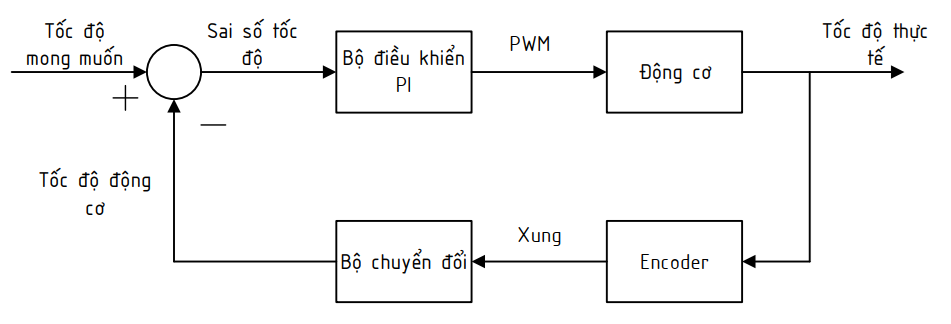
\includegraphics[width=0.8\textwidth]{pictures/chapter6/PI_controller.png}
                    \caption{Sơ đồ khối bộ điều khiển động cơ}
                    \label{PI_controller}
               \end{figure}
          \begin{itemize}
               \item Thời gian xác lập: $T_s \leq 0.2 \,\mathrm{s}$;
               \item Độ vọt lố: $\%OS \leq 2 \%$.
          \end{itemize}
          \hspace*{0.6cm}Sử dụng công cụ PID Tuner Toolbox của MATLAB, thực hiện điều chỉnh các hệ số PID để đạt được yêu cầu thiết kế
          \begin{itemize}
               \item \textit{Động cơ 1:} Hàm truyền động cơ 1 (động cơ bánh phải)
               \begin{figure}[H]
                    \centering
                    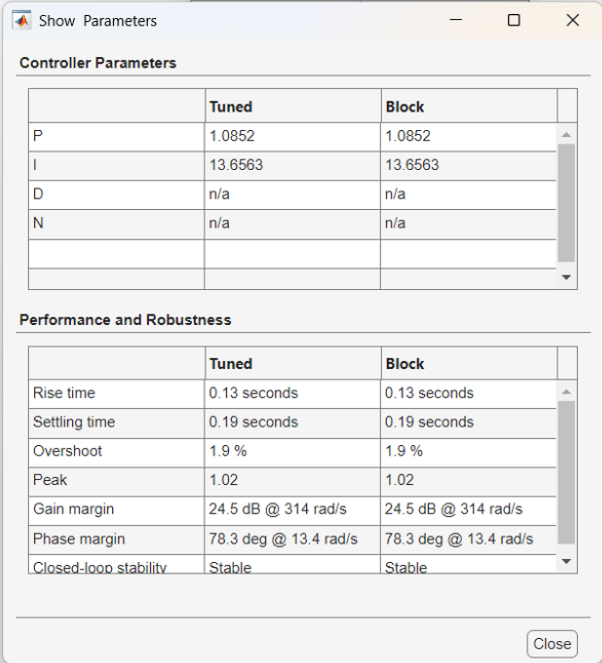
\includegraphics[width=0.6\textwidth]{pictures/chapter6/params_JGB1.png}
                    \caption{Thông số bộ điều khiển động cơ bánh phải}
                    \label{params_JGB1}
               \end{figure}
               \hspace*{0.6cm}Ta có các hệ số PI như sau với thời gian xác lập 0.19 s:
               \begin{equation*}
                    \begin{cases}
                         &K_P = 1.0852 \\ 
                         &K_I = 13.6563
                    \end{cases}
               \end{equation*} 
               \item \textit{Động cơ 2:} Hàm truyền động cơ 2 (động cơ bánh trái)\\
               \begin{figure}[H]
                    \centering
                    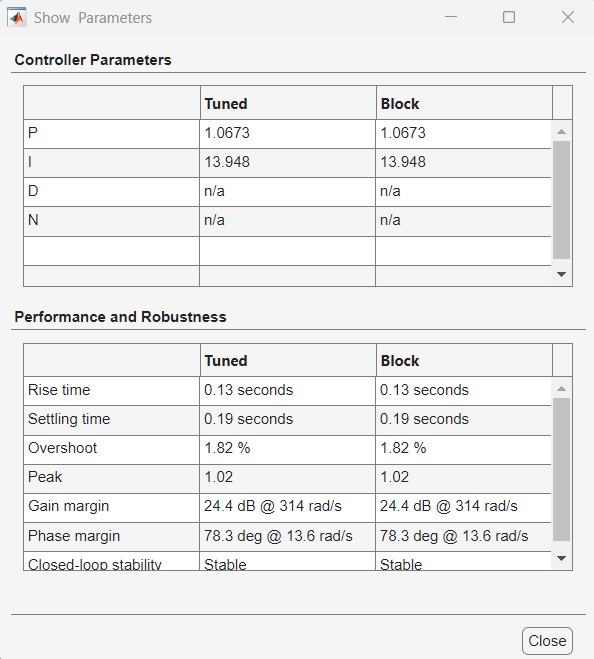
\includegraphics[width=0.6\textwidth]{pictures/chapter6/params_JGB2.png}
                    \caption{Thông số bộ điều khiển động cơ bánh trái}
                    \label{params_JGB2}
               \end{figure}
               \hspace*{0.6cm}Ta có các hệ số PI như sau với thời gian xác lập 0.19 s:
               \begin{equation*}
                    \begin{cases}
                         &K_P = 1.0673 \\ 
                         &K_I = 13.948
                    \end{cases}
               \end{equation*} 
          \end{itemize}

          

